%\section{Electrical aspects}

\section{Electronics}
Our electronics were designed to handle all low-level tasks that are
required to move AquaTux, acquire sensor data from the IMU and depth sensors. 
The main goal of the electronics is to allow the AUV to be driven with only
high-level heading and depth commands. The electronics are responsible for
executing the commands and controlling their results (e.g. depth or
heading) in a ``black box'' fashion. The electronics are managed by the embedded
system described in the next section, giving access to each electronic peripheral.

Aquatux's electronics are arranged in two stacks of PCBs, one dedicated to power 
distribution and management, and the ``main stack'', which breaks out the on board 
FPGA's I/Os to any number of children.

\subsection{Main Stack}
At the heart of Aquatux's electronic subsystem is a Terasic DE0-Nano, a small 
form-factor FPGA development board, containing an Altera Cyclone IV FPGA. The 
DE0 mates directly to the ``Interface Board'' which breaks out all of the 
available I/0s to a 120 pin board to board connector (Figure~\ref{mstack}). Any number of new PCBs 
can be mated, by providing the mating male and female connectors. These 
connectors form a wide bus between the FPGA and the mating boards, which when 
coupled with the reconfigurability of an FPGA, makes it very easy to incorporate 
new PCBs without having to physically rewire parts of the submarine -- a Quartus 
recompile is all that's required. The interface board also connects to the IMU, 
a VectorNav VN-100 Rugged, which performs its own sensor signal processing to 
output attitude data to the FPGA.

\begin{figure}
\begin{center}
 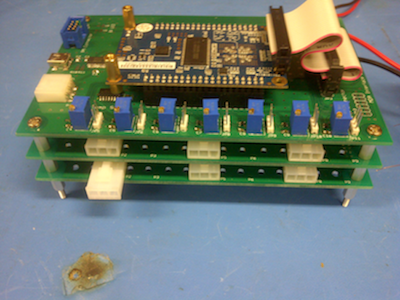
\includegraphics[width=3in]{fig/main_stack.png} %1.34
\vspace{.05in}
\hrule
\caption{The main stack connector. Top, the interface board and DE0 nano. Below, two 6 channel motor drivers.}\label{mstack}
\end{center}
\end{figure}

\subsection{Motor Board}

The motor boards are used to control the Seabotix BTD150 Thrusters used on AquaTux 
and other actuators internal to the submarine. Each motor board (Figure~\ref{motorb}) consists of 6 NMOS 
high-side half bridges driven by Linear Technologies LT1660 half-bridge drivers. 
Each half bridge has a sister with which it can be used a full bridge, by soldering 
the output connector in the correct position. Complementary PWM inputs to each driver 
can be sourced from one of three sets of I/Os provided via the main stack connector, 
allowing a multiplicity of boards to be mated to the stack. Presently, two of three 
boards are used, providing the five full bridges required to drive Aquatux's motors. 
The final board is provision to drive internal peripherals such as marker droppers in 
future competitions.

\begin{figure}
\begin{center}
 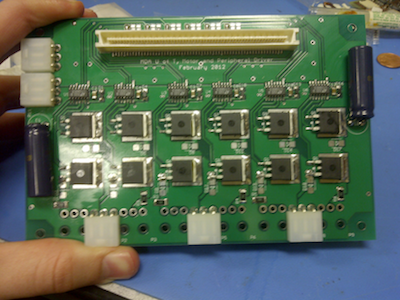
\includegraphics[width=3in]{fig/motor_board.png} %1.34
\vspace{.05in}
\hrule
\caption{A motor board, configured with 3 full bridges.}\label{motorb}
\end{center}
\end{figure}

\subsection{Power Distribution}
Power for Aquatux's electronic systems, excluding the netbook, is provided by 
two 24V NiMH battery packs. The power distribution board switches the battery 
voltage with a relay, which is controlled by the FPGA's soft-processor. 
Throwing the kill switch (by removing the velcroed handle on the side of the 
hull) opens a reed switch which breaks the relay's coil current. Three DC/DC 
converters (3.3V, 5V, 12V) source from this voltage, and form a stack of PCBs 
with the power management board above them. LC output filters on power management 
board remove switching harmonics, before breaking out the rail voltages to the 
submarine through a series of copper bus-bars. Four pairs of analog comparators 
alert the FPGA when any of the rails over or under-volts by 5 percent of their nominal 
voltage. As a final baseline precaution, breakers have been inserted between the 
batteries and relay, and between the power management board and bus-bars for each rail.

\subsection{Power Source}
The NiMH battery packs were custom designed by our team: each pack is
composed of 20 SY136T Sanyo nickel metal hydride batteries. All
batteries are connected in series to form a 24V nominal battery pack
with a capacity of 4100mAh. Temperature sensors embedded in each pack allow 
the FPGA to kill the sub if any one pack overheats.
